\documentclass[twocolumn,amsmath,amssymb,aps]{revtex4}
\usepackage{graphicx}% Include figure files
\usepackage{dcolumn}% Align table columns on decimal point
\usepackage{bm}% bold math
\usepackage{color, subfigure}
\usepackage{csquotes}





\begin{document}
\title{Order and Chaos in Nonlinear Physics\\
	 An Overview of the Lorenz System and the Logistic Map}%
\author{Huan Q, Bui}\email{hqbui21@colby.edu}
\affiliation{Departent of Physics and Astronomy, Colby College.}
\date{\today}
\begin{abstract}
This paper reviews the emergence of ``chaos'' in nonlinear science through numerical simulations of the Lorenz System. Following Lorenz' groundbreaking 1963 paper, we show that chaos is deterministic and contains regular structures. Conversely, we will also show, via the logistic map, that chaos can also emerge from very simple governing dynamics.
\end{abstract}
\maketitle




\section{Introduction}
\textit{Chaos} in the technical sense refers to dynamical systems whose seemingly irregular and random behaviors are governed by deterministic law and are extremely sensitive to initial conditions. While it might seem counter-intuitive to the reader that determinism is one of the defining factors of chaos, there are in fact many such systems in nature. In hydrodynamics, the weather is a prime example: a collection of particles following deterministic rules as simple as momentum and energy conservation can manifest in behaviors so complex that even the most powerful computers cannot predict with certainty whether the coming fortnight will be cloudy or clear.  


The essence of chaos theory is perhaps best summarized by Edward Lorenz -- one of the pioneers of the field:
\begin{displayquote}
``Chaos: When the present determines the future, but the approximate present does not approximately determine the future.''\cite{lorenz_quote}
\end{displayquote}
Chaos theory emerged in the 1960s following a number of discoveries in physics and mathematics, including Lorenz' famous paper titled ``Deterministic Nonperiodic Flow.'' In this paper, Lorenz explores a simplified  model for atmospheric convection consisting of three coupled ordinary differential equations. Now known as the \textit{Lorenz} \textit{system}, this model exhibits not only nonlinear and nonperiodic behavior, but also extreme sensitivity to perturbations in initial conditions characteristic of chaos. In Section I, we will study the chaotic behavior of this system in detail. We will also see that, surprisingly, there is also a sense of regularity in the chaos. 


Following Lorenz' discovery, Robert May extended the boundary of chaos theory through his work on the logistic difference equation (now known as the logistic map) in his 1976 paper ``Simple mathematical models with very complicated dynamics.'' \cite{rmay76} Starting with a very simple rule which resembles the regularity that emerges from the Lorenz system, Robert May showed that highly chaotic behaviors can in fact emerge. In Section II, we will explore these chaotic behaviors in more detail. We will also touch on some interesting and beautiful mathematical connections.

Robert May's result corresponds nicely with Lorenz'. On the one hand, starting with a rather complex set of differential equations, Lorenz discovered chaos and an underlying regularity within the apparently random behavior. On the other, Robert May created chaos out of a similar rule which emulates the regularity mentioned before. Together, these show something deeply curious and counter-intuitive about chaos.




\section{From Chaos to Order}
In this section, we consider the Lorenz equations, an exemplary system that possesses chaotic dynamics. We will also discover a glimpse of order within the seemingly erratic behaviors of the system.  
\subsection{The Lorenz System}
The Lorenz system is given by the following set of coupled differential equations.\cite{flow}
\begin{eqnarray}
\dot{X} &=& \sigma(Y-X)\nonumber\\
\dot{Y} &=& r X - Y - XZ\nonumber\\
\dot{Z} &=& XY - bZ\nonumber.
\end{eqnarray}
Here, the model parameters $\sigma, r, b$ are physical constants that characterize the properties of the fluids and how they interact. We pay attention in particular to the parameter $r$, which is proportional to the Rayleigh number. Since the Lorenz system is based on a model for convection, the Rayleigh number pays an important role. As we will see, the system exhibits markedly distinct behaviors when $r$ lies within different regimes.

\subsection{Prelude to the Emergence of Chaos}

Assume that $\sigma,b$ are fixed. We now see how the Lorenz system evolves from the initial condition $(X,Y,Z) = (0, 1, 2)$ as $r$ changes. First, let us consider the steady state solutions when $r\in [0,4]$, shown in Figure \ref{fig:lorenz_2}.
\begin{figure}[!htb]
	\centering
	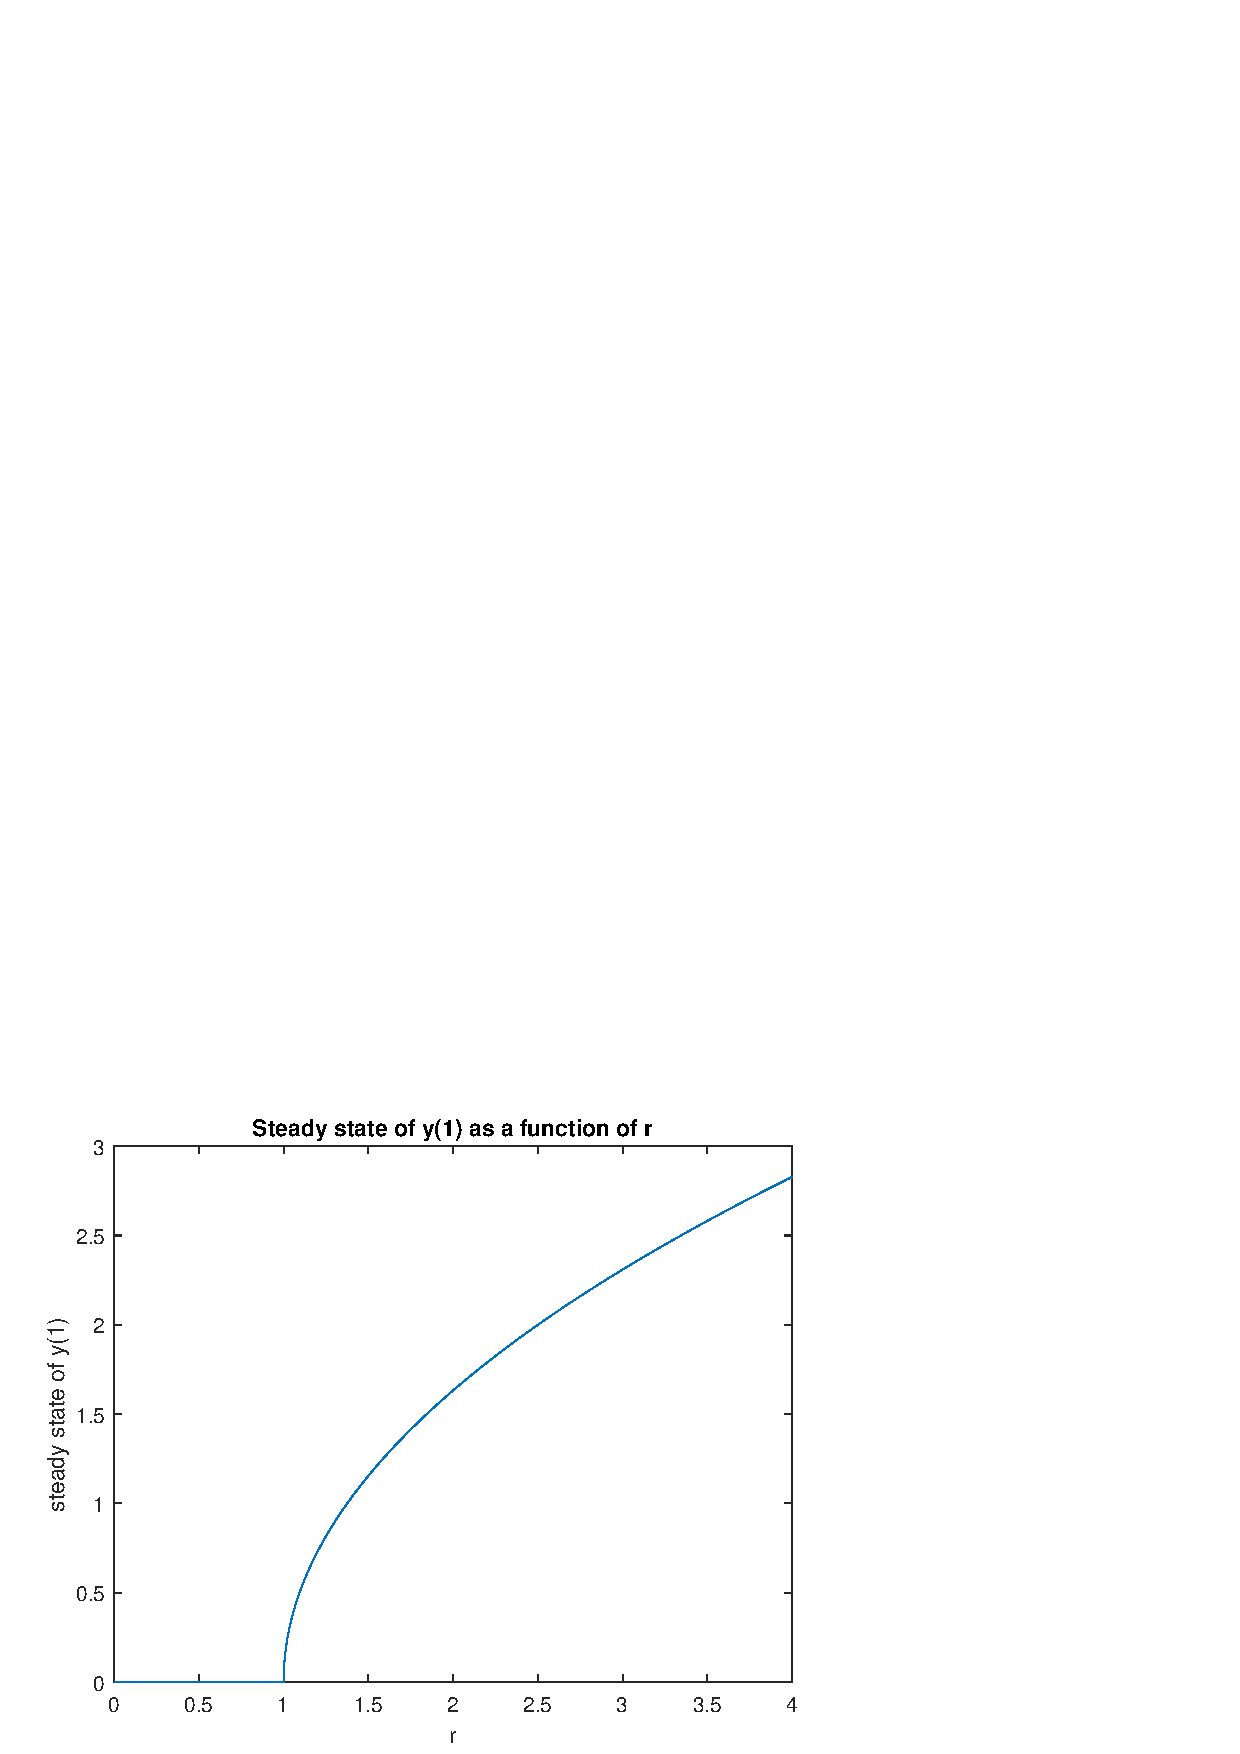
\includegraphics[scale=0.5]{bifurcation_sharp}
	\caption{Steady state values for $X$ when $r\in [0,4]$. The system starts at $(X,Y,Z) = (0,1,2)$.}
	\label{fig:lorenz_2}
\end{figure}


When $r \in [0,1)$, $X$ does not leave $0$. However, when $r \geq 1$, we start to see an increase in the steady state of $X$. Recall that $r$ is related to the Rayleigh number in the convection model. In this context, the point $r = 1$ corresponds to the onset of convection. When the Rayleigh number increases beyond $1$, the convection gets more and more violent. This corresponds to the increasing stead-state of $X$. 
\begin{figure}[!htb]
	\centering
	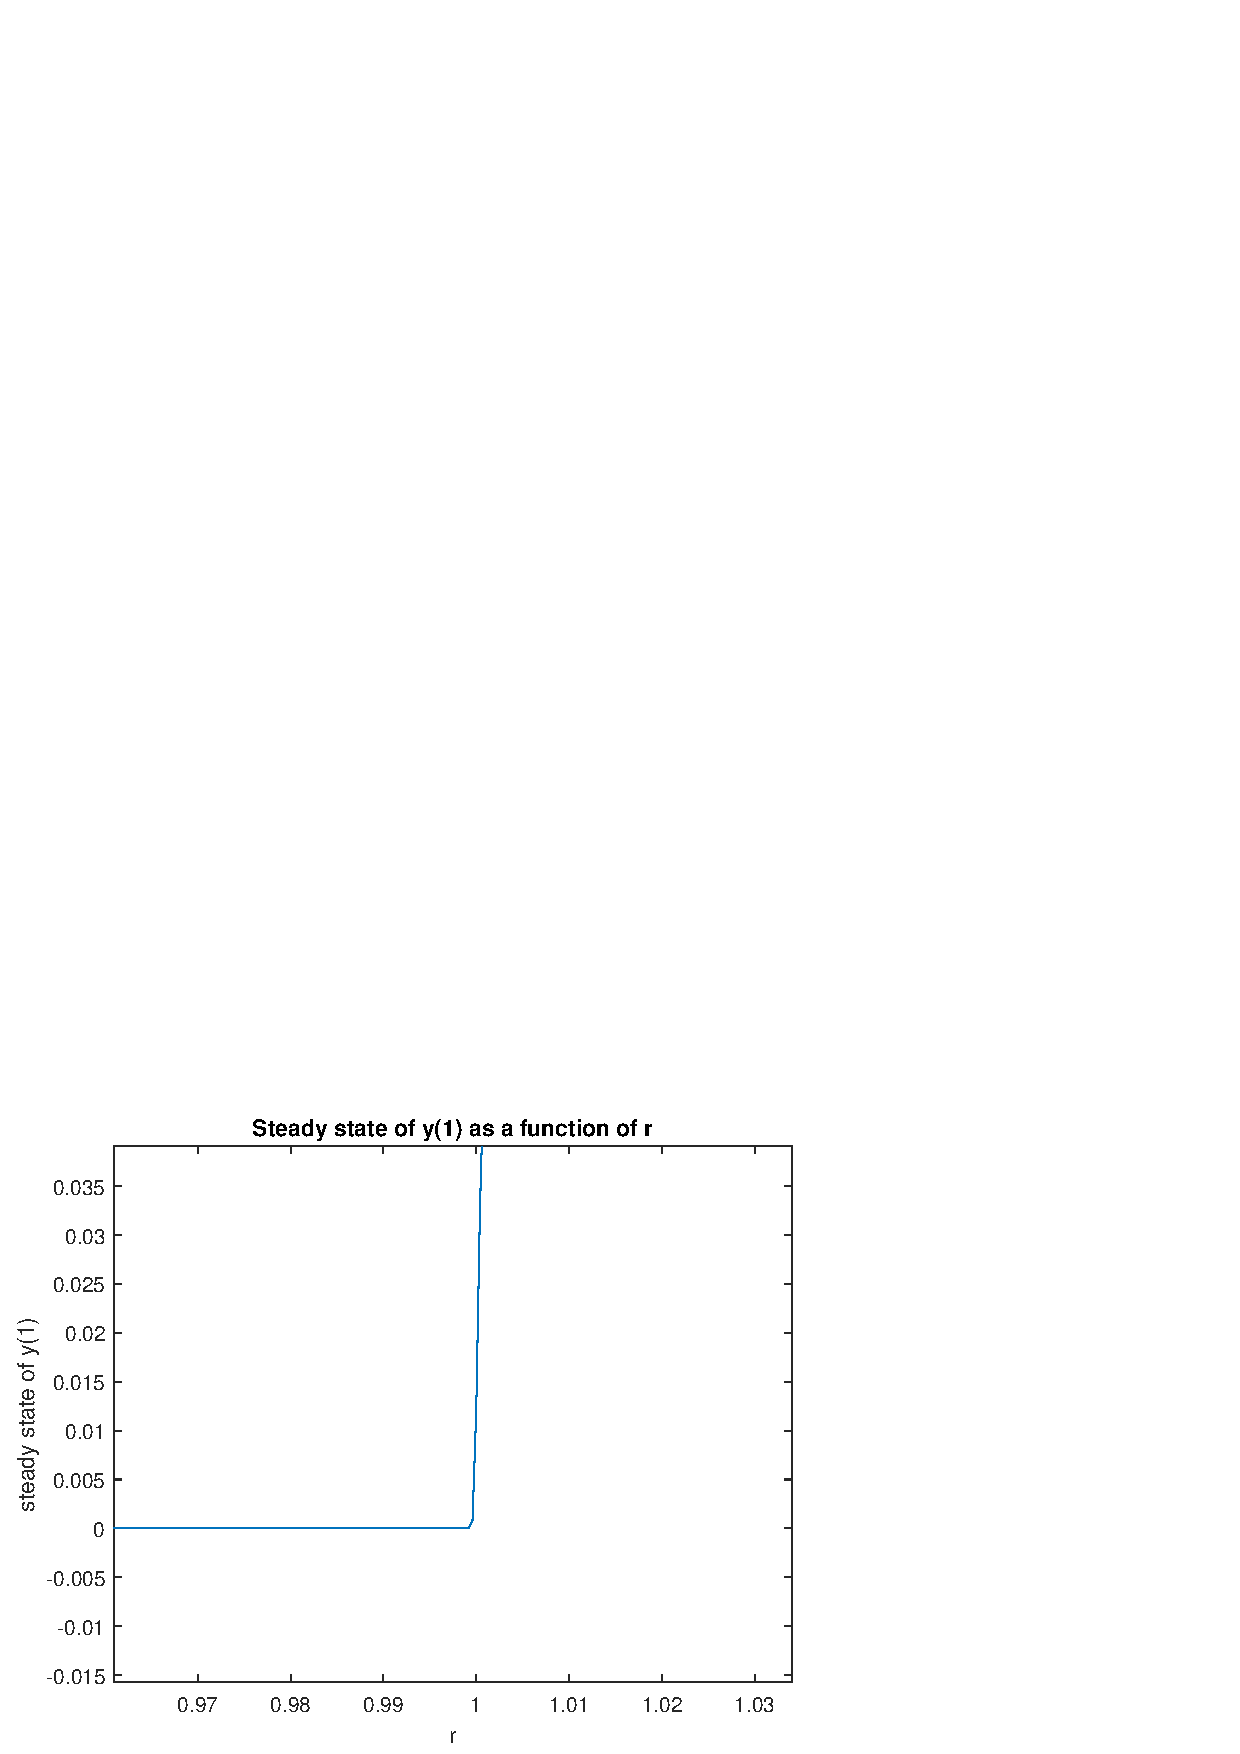
\includegraphics[scale=0.5]{bifurcation_sharp_corner}
	\caption{The steady state of $X$ undergoes an abrupt change as $r$ increases past the value $1$.}
	\label{fig:lorenz_3}
\end{figure}

Careful analysis shows we can view $r = 1$ as a threshold for the Lorenz system. Figure \ref{fig:lorenz_3} shows that the steady state of $X$ undergoes an abrupt change as $r$ increases past the value $1$. The slight curvature is due to the limited time range in the MATLAB solver. The reader can check that when the time range gets arbitrarily large, the rate of change of $X_{\text{steady state}}$ with respect to $r$ is infinite at $r=1$. 

\subsection{Emergence of Chaos}
One might expect that as $r$ grows beyond $1$, the steady state of $X$ continues to increase following the trajectory in Figure \ref{fig:lorenz_2}. However, this is not the case. 
\begin{figure}[!htb]
	\centering
	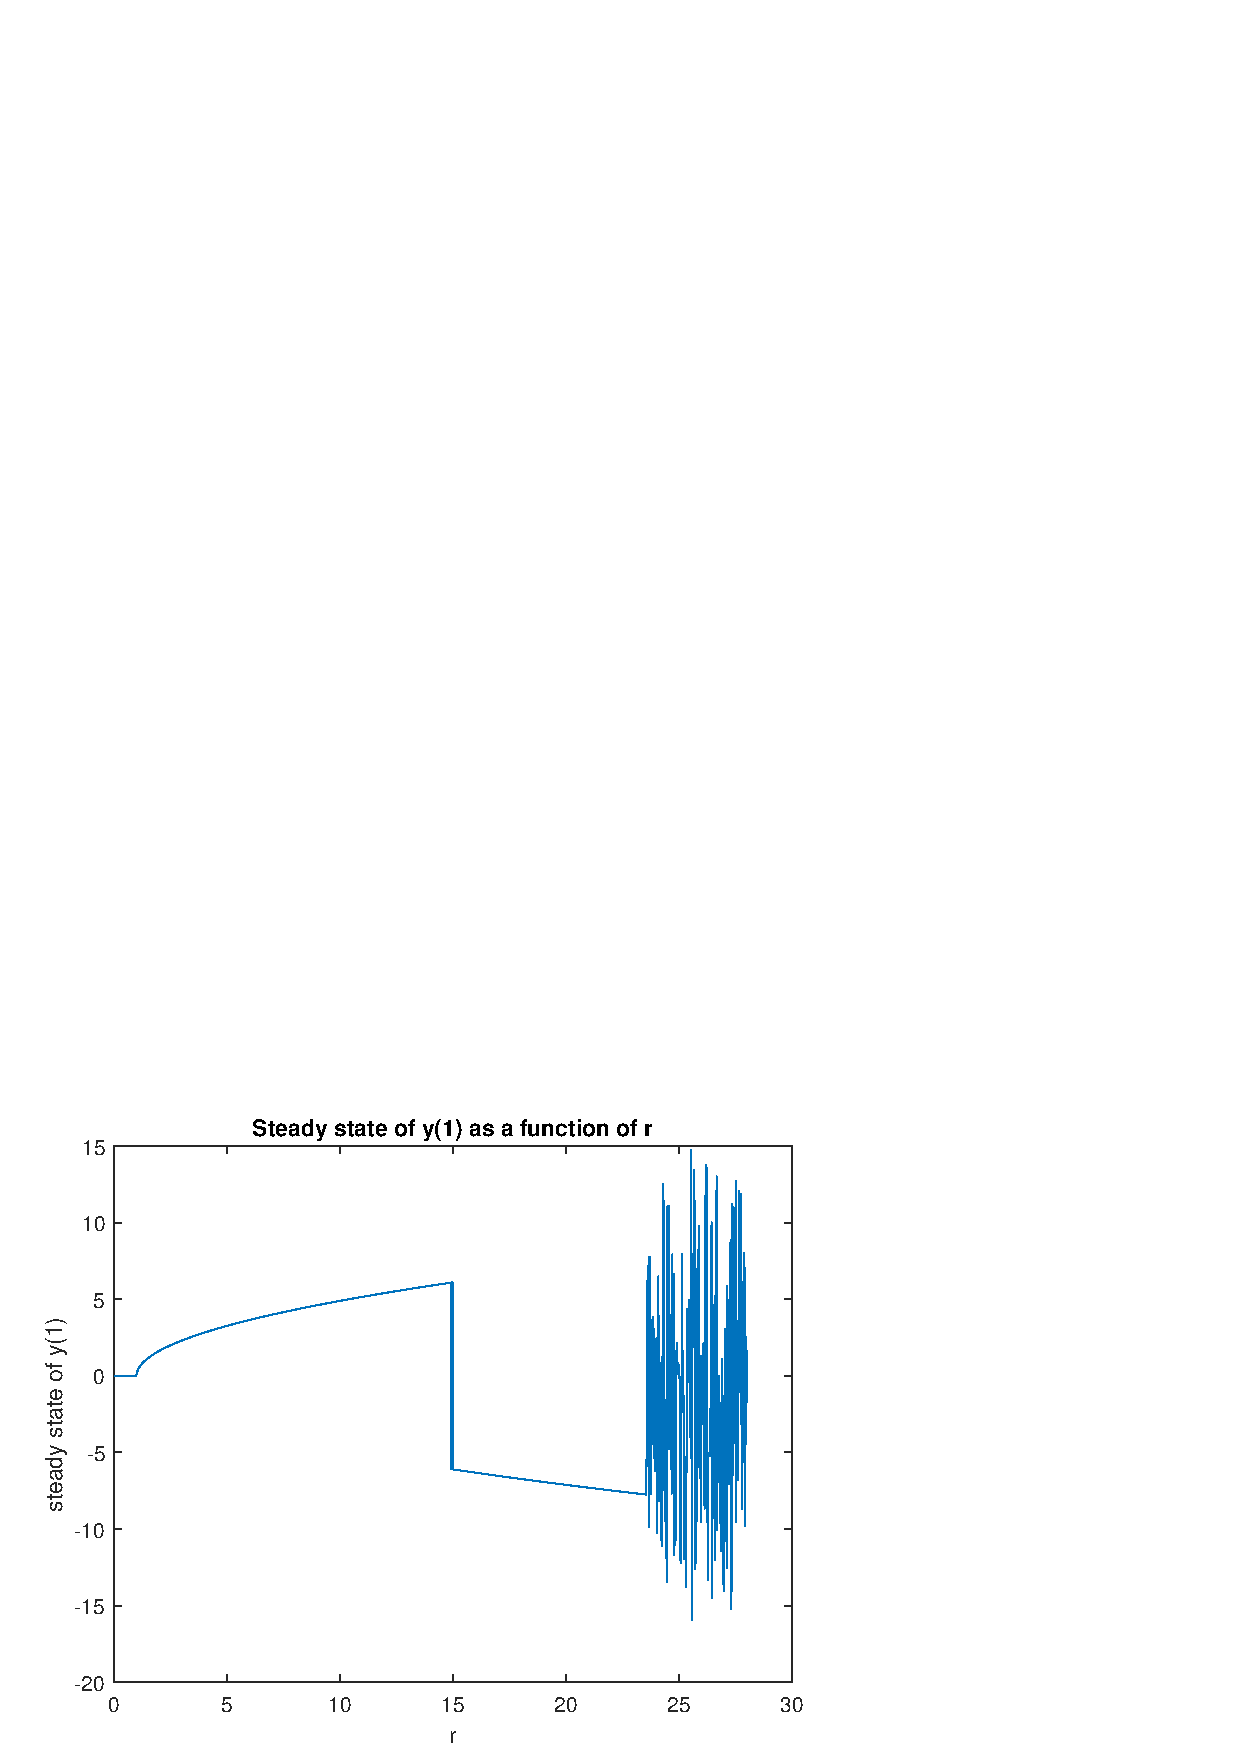
\includegraphics[scale=0.5]{bifurcation_chaos}
	\caption{blah}
	\label{fig:bifurcation_chaos}
\end{figure}

Figure \ref{fig:bifurcation_chaos} shows an abrupt drop and strong oscillations in $X_{\text{steady state}}$ as when $r \approx 15$, followed by decrease towards a region of erratic, highly oscillatory behavior at $r\approx 23.3$. We notice that the oscillations are also highly nonperiodic. To see this better, we can go to phase space. Let $r=28$ and consider the initial condition $(0,0.001,0)$. Figure \ref{fig:lorenz_butterfly_1} shows the phase trajectory projected onto the $Z-X$ plane.  
\begin{figure}[!htb]
	\centering
	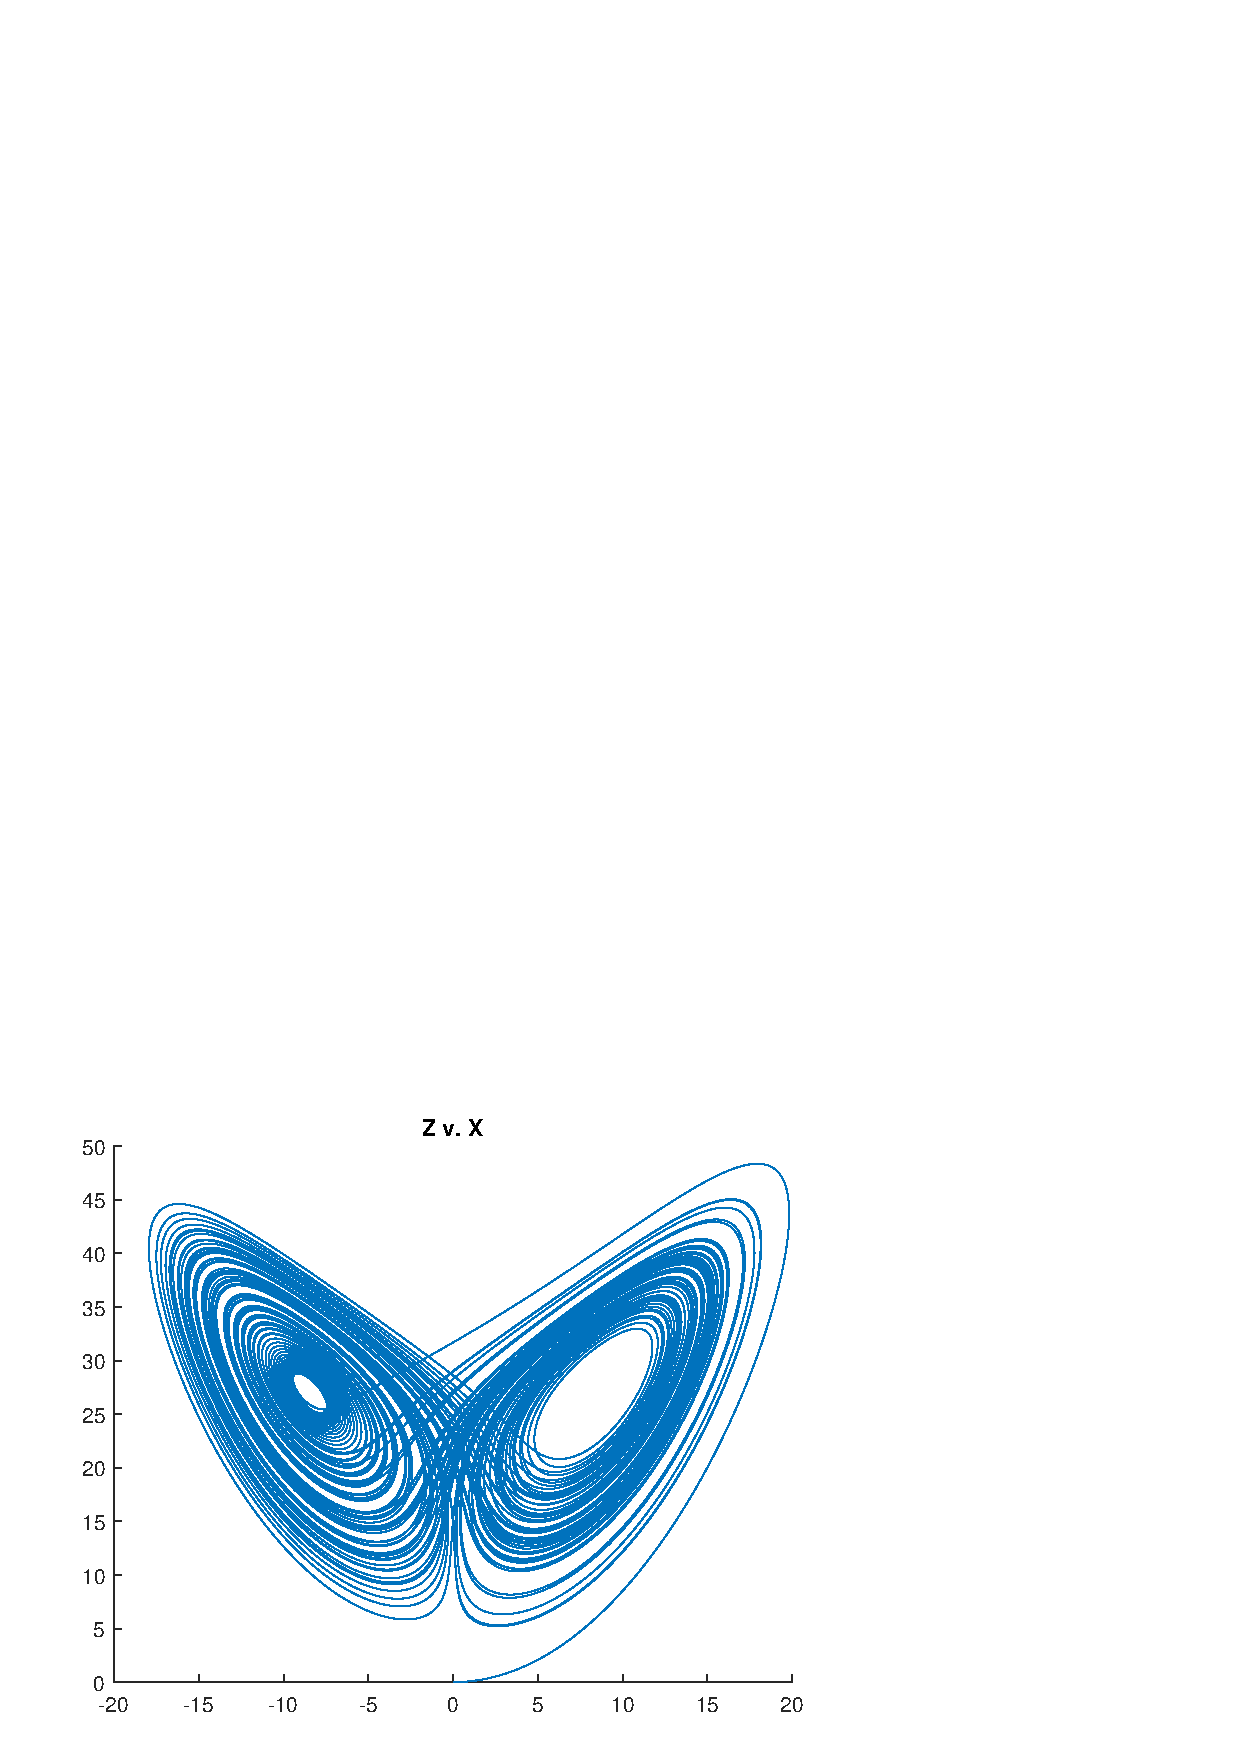
\includegraphics[scale=0.5]{ZX_butterfly}
	\caption{Phase trajectory projected onto the $Z-X$ plane. $r=28$ and initial condition $(0,0.001,0)$.}
	\label{fig:lorenz_butterfly_1}
\end{figure}

It is clear that there the solution is highly oscillatory with highly irregular amplitudes. We also notice that even though the trajectory does not converge to neither a curve nor a point, it is very well-confined within a butterfly-shaped set of points on the $Z-X$ plane. It turns out that for sufficiently large time, the trajectory eventually fills the space outlined by the boundary of the ``butterfly.'' This is an example of a special kind of attractor called the \textit{strange attractor}. Now, we further see how \textit{strange} this attractor is by considering a very small perturbation from the initial condition $(0,0.001,0)$ in Figure \ref{fig:lorenz_butterfly_2}.
\begin{figure}[!htb]
	\centering
	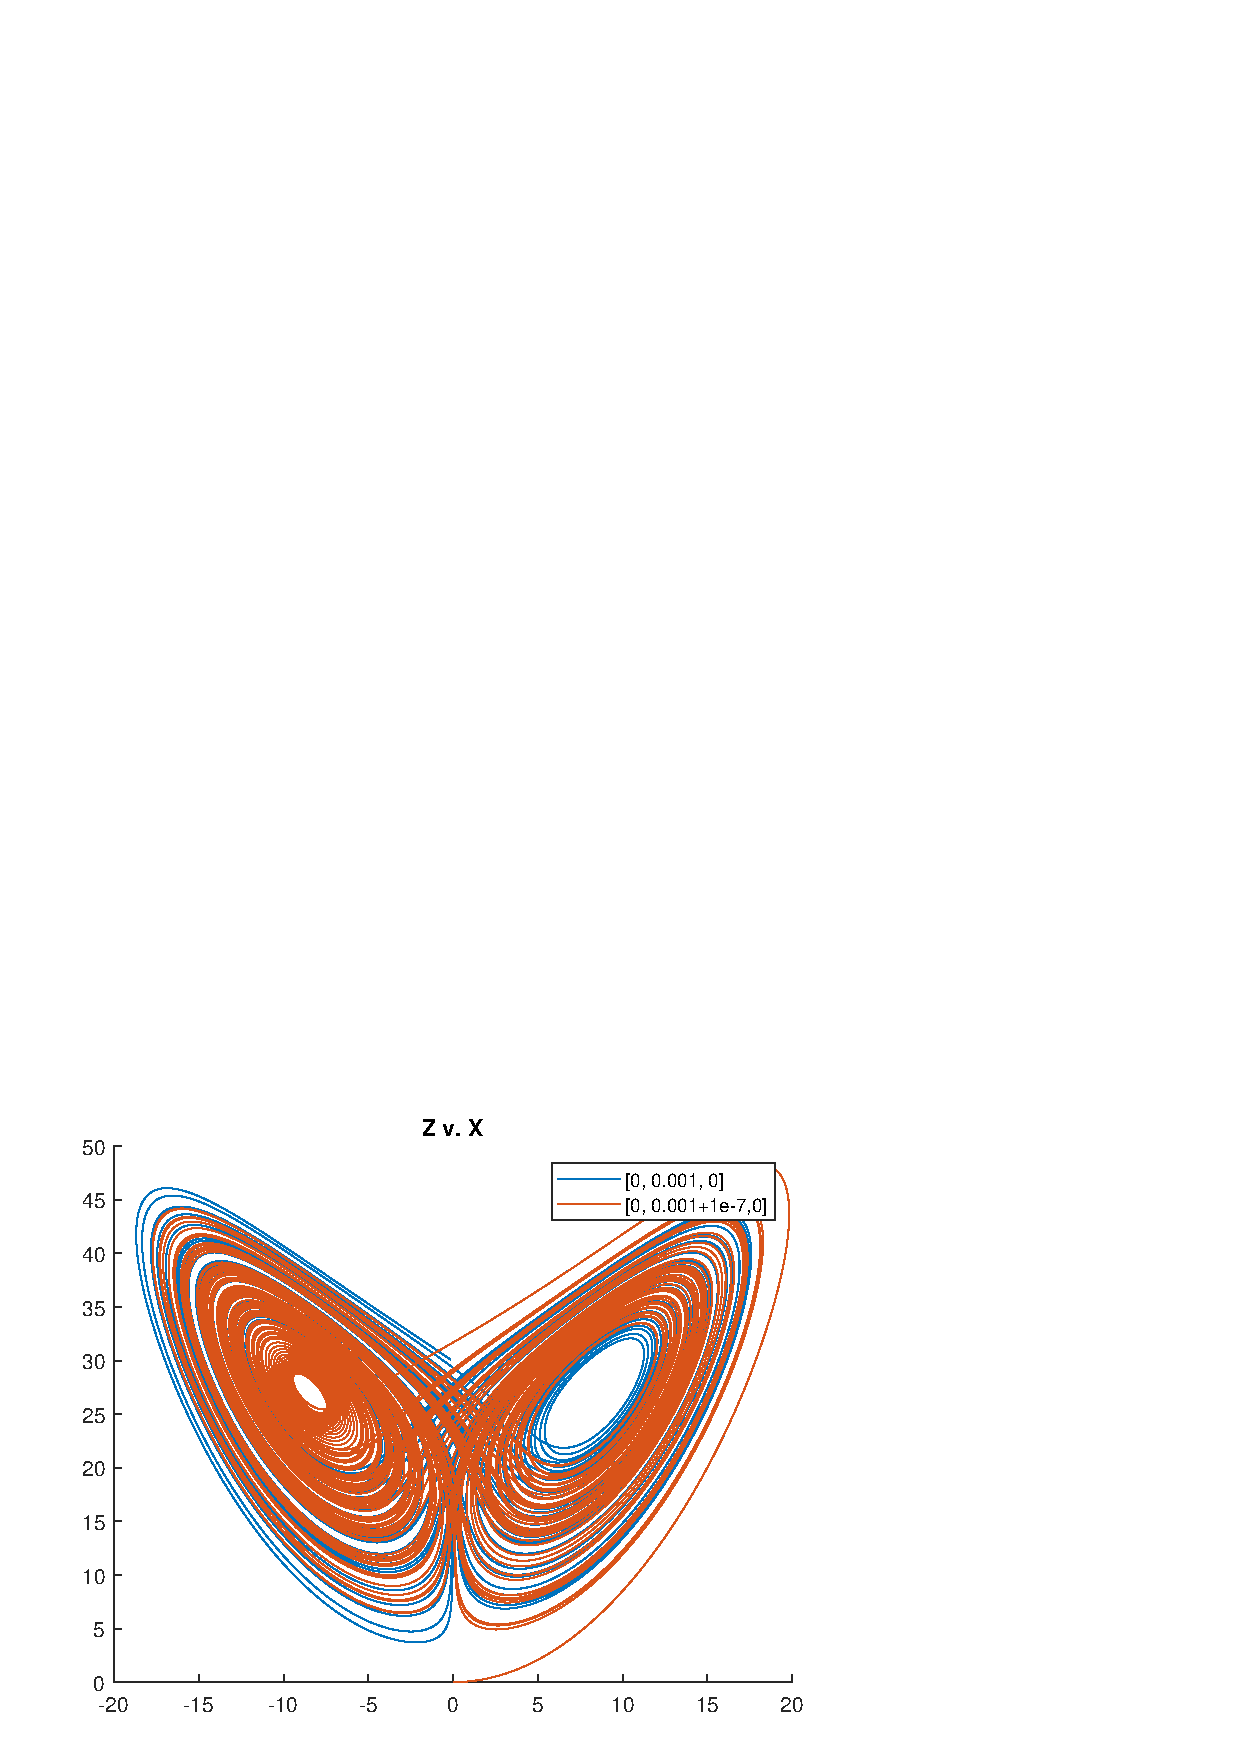
\includegraphics[scale=0.5]{ZX_butterfly_sensitive}
	\caption{Phase trajectories projected onto the $Z-X$ plane. $r=28$ and initial condition $(0,0.001,0)$ (blue) and $(0,0.001+10^{-7},0)$ (orange).}
	\label{fig:lorenz_butterfly_2}
\end{figure}
Figure \ref{fig:X_sensitive_1} shows the difference between the solutions for $X$ for the initial condition $(0,0.001,0)$ and $(0,0.001+10^{-7},0)$. 
\begin{figure}[!htb]
	\centering
	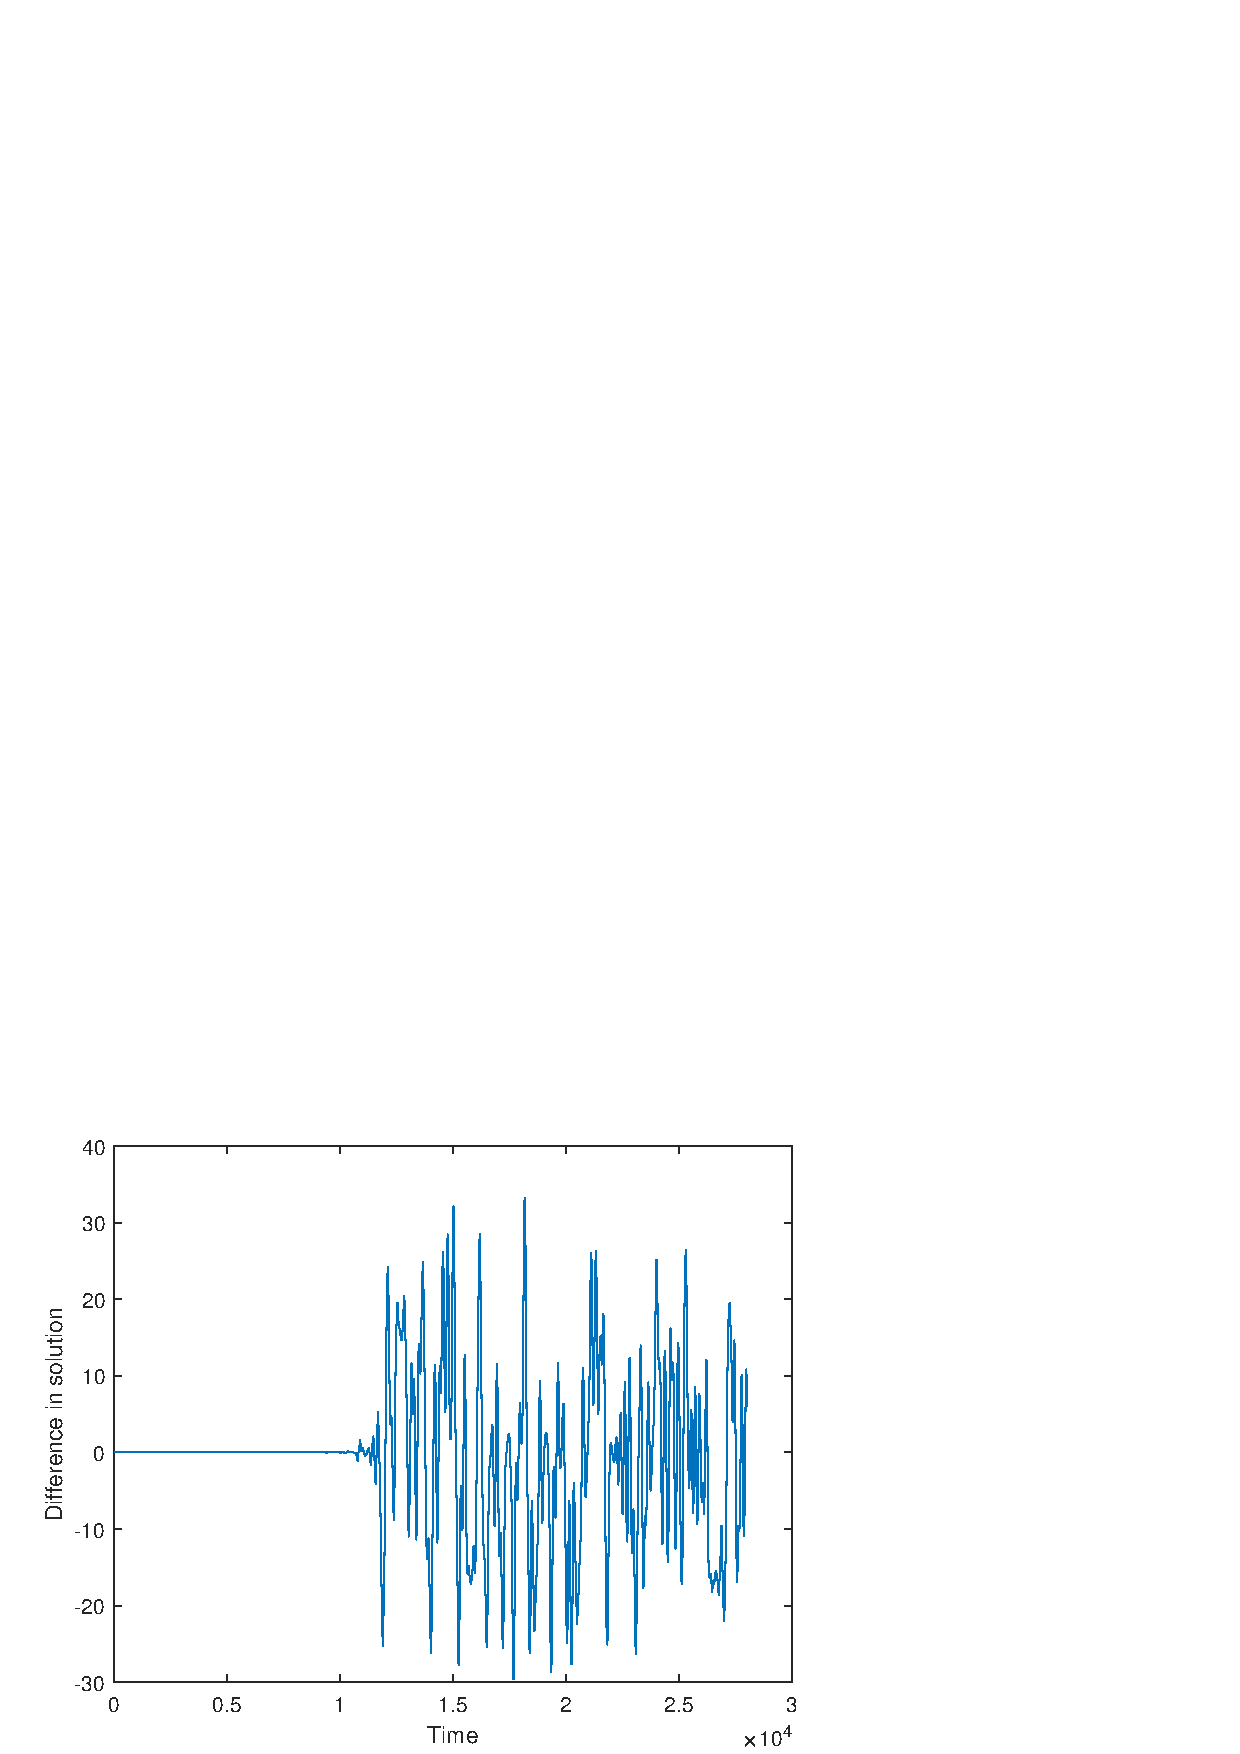
\includegraphics[scale=0.5]{difference_init}
	\caption{blah}
	\label{fig:X_sensitive_1}
\end{figure}
Initially, the solutions corresponding these slightly different initial conditions behave very similarly: the orange and blue phase trajectories overlap very well up to around $t\approx 10^{4}$. After this, the solutions evolve in completely different behaviors. However, we notice that these solutions are still confined within the ``butterfly.'' This is an example of a more general fact: for any arbitrary close initial conditions, phase trajectories can get arbitrarily far from each other (while, of course, still remaining a confined region defined by the strange attractor). Conversely, it is also true that initial conditions that are arbitrarily far apart (again, within the same confined region) will evolve to be arbitrarily close at some point. This is what so \textit{strange} about the strange attractor: it is locally unstable but globally stable. 

What we have seen so far is chaos: apparently random behaviors that are in fact deterministic and are extremely sensitive to initial conditions. Next, we look at a subtle underlying regularly within chaotic solutions beyond the governing differential equations.






\subsection{Regularity in Chaos}

Consider the time evolution of $X$ in Figure \ref{fig:time_evolve}.
\begin{figure}[!htb]
	\centering
	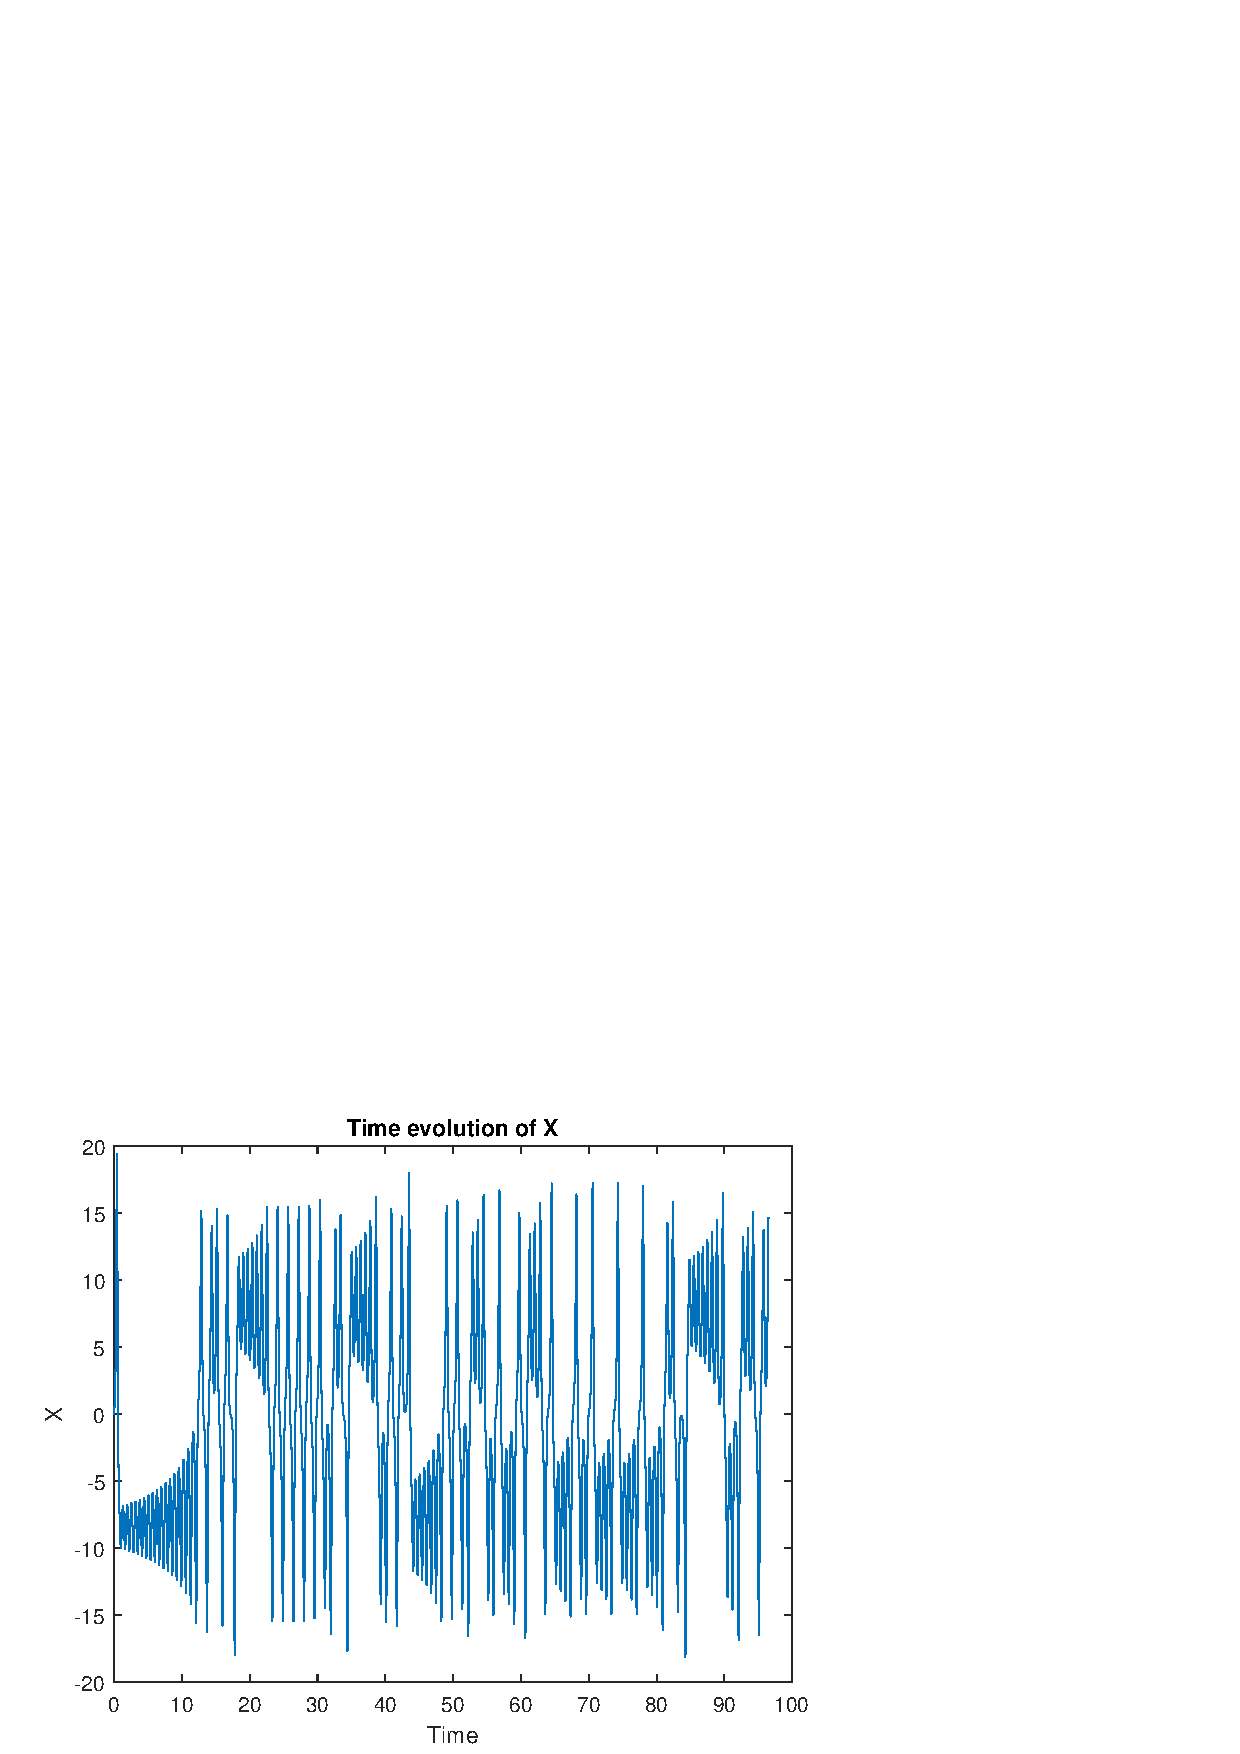
\includegraphics[scale=0.5]{time_evolve}
	\caption{Blah}
	\label{fig:time_evolve}
\end{figure}
We notice a pattern in how the peaks appears. To characterize this, we follow Lorenz' work and consider the \textit{Poincar\'{e} section} given in Figure \ref{fig:poincare_1}.
\begin{figure}[!htb]
	\centering
	\includegraphics[scale=0.4]{Poincare_section}
	\caption{$r = 28$}
	\label{fig:poincare_1}
\end{figure}

This is very strong evidence for a sense of order in the chaotic solution. In functional form, we can write
\begin{equation*}
Z_{k+1} = f(Z_k)
\end{equation*}
where $Z_{k+1}$ is the value of the $(k+1)$th peak following the $Z_{k}$ maximum. While not exact, this function tells us roughly what the next peak in $X$ be given some peak in $X$. (\textcolor{red}{this sounds weird... I need to rephrase this.})



\section{From Order to Chaos}
\subsection{The Logistic Map}
Having seen how chaotic behaviors in the Lorenz system in fact follow a regular pattern, it would be tempting for us to now ask whether given a rule of the form 
\begin{equation*}
Z_{k+1} = f(Z_k),
\end{equation*}
whether it is possible to generate chaos. The answer turns out to be affirmative. In this section, we consider the logistic map of the form
\begin{equation*}
x_{k+1} = ax_k(1-  x_k)
\end{equation*}
where $a \in [0,4]$. When $x_{k+1}$ is plotted against $x_{k}$, we get a concave-down parabolic Poincar\'{e} section. Qualitatively, this Poincar\'{e} section is similar to that in the preceding section. However, it is easier to deal with mathematical since it can be written in a non-piecewise 
closed form. \textcolor{red}{Perhaps mention some history... e.g. ecology, population dynamics, how it's derived from the logistic equation, and how it can be pathological. etc.}

Note how simple this rule is, especially in comparison to the Lorenz system. There is only one variable, whereas the Lorenz system has three. There is also only one model parameter. 


\subsection{Period-Doubling Cascades}
To see whether this rule generates chaotic behavior, let us look at the bifurcation diagram again where the varying parameter is $a$. Figure \ref{fig:logistic_2} shows the full bifurcation diagram. 
\begin{figure}[!htb]
	\centering
	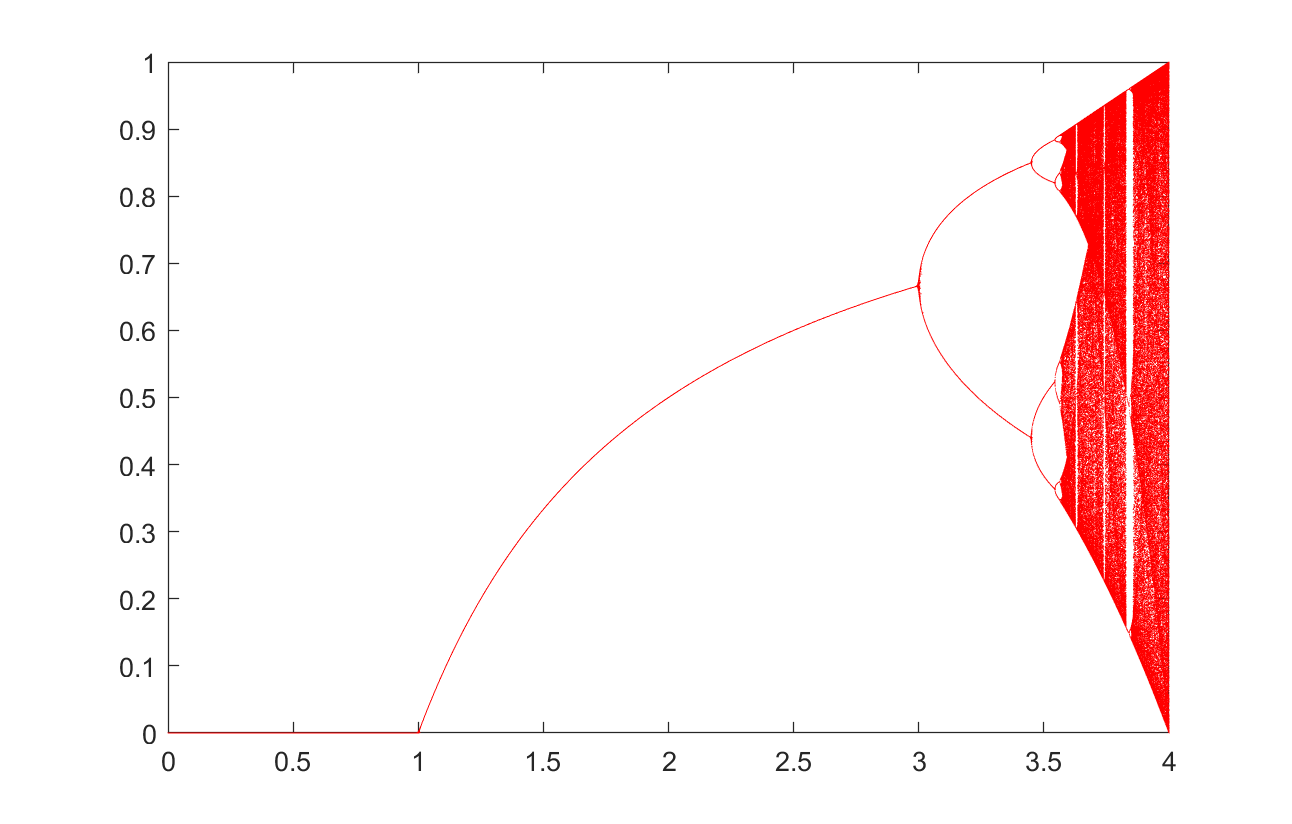
\includegraphics[scale=0.25]{logistic_2.png}
	\caption{Full bifurcation diagram, $a \in [0,4]$.}
	\label{fig:logistic_2}
\end{figure}


The behavior when $a$ goes from $0$ to $3$ is similar to what we saw before. However, notice the pitchfork bifurcation at $a= 3$, followed by one ``second-order'' pitchfork bifurcation at each branch. This tells us that for $a \in [3,3.5]$, the steady state solution converges to an oscillation between two values. When $a$ gets larger, the steady state solution oscillates between 4 values (Figure \ref{fig:logistic_2}).

Continue zooming in, we can see that the steady state oscillates between 8 values (Figure \ref{fig:logistic_3}), 16 (Figure \ref{fig:logistic_4}. Here, each of the 8 branches has a pitchfork bifurcation to a total of 16 branches), then 32 (Figure \ref{fig:logistic_5}), and so on. Thus, we see that it is possible to generate highly complex dynamics from a very simple rule.

\textcolor{blue}{Discuss the 1,3,5 periods...}



\begin{figure}[!htb]
	\centering
	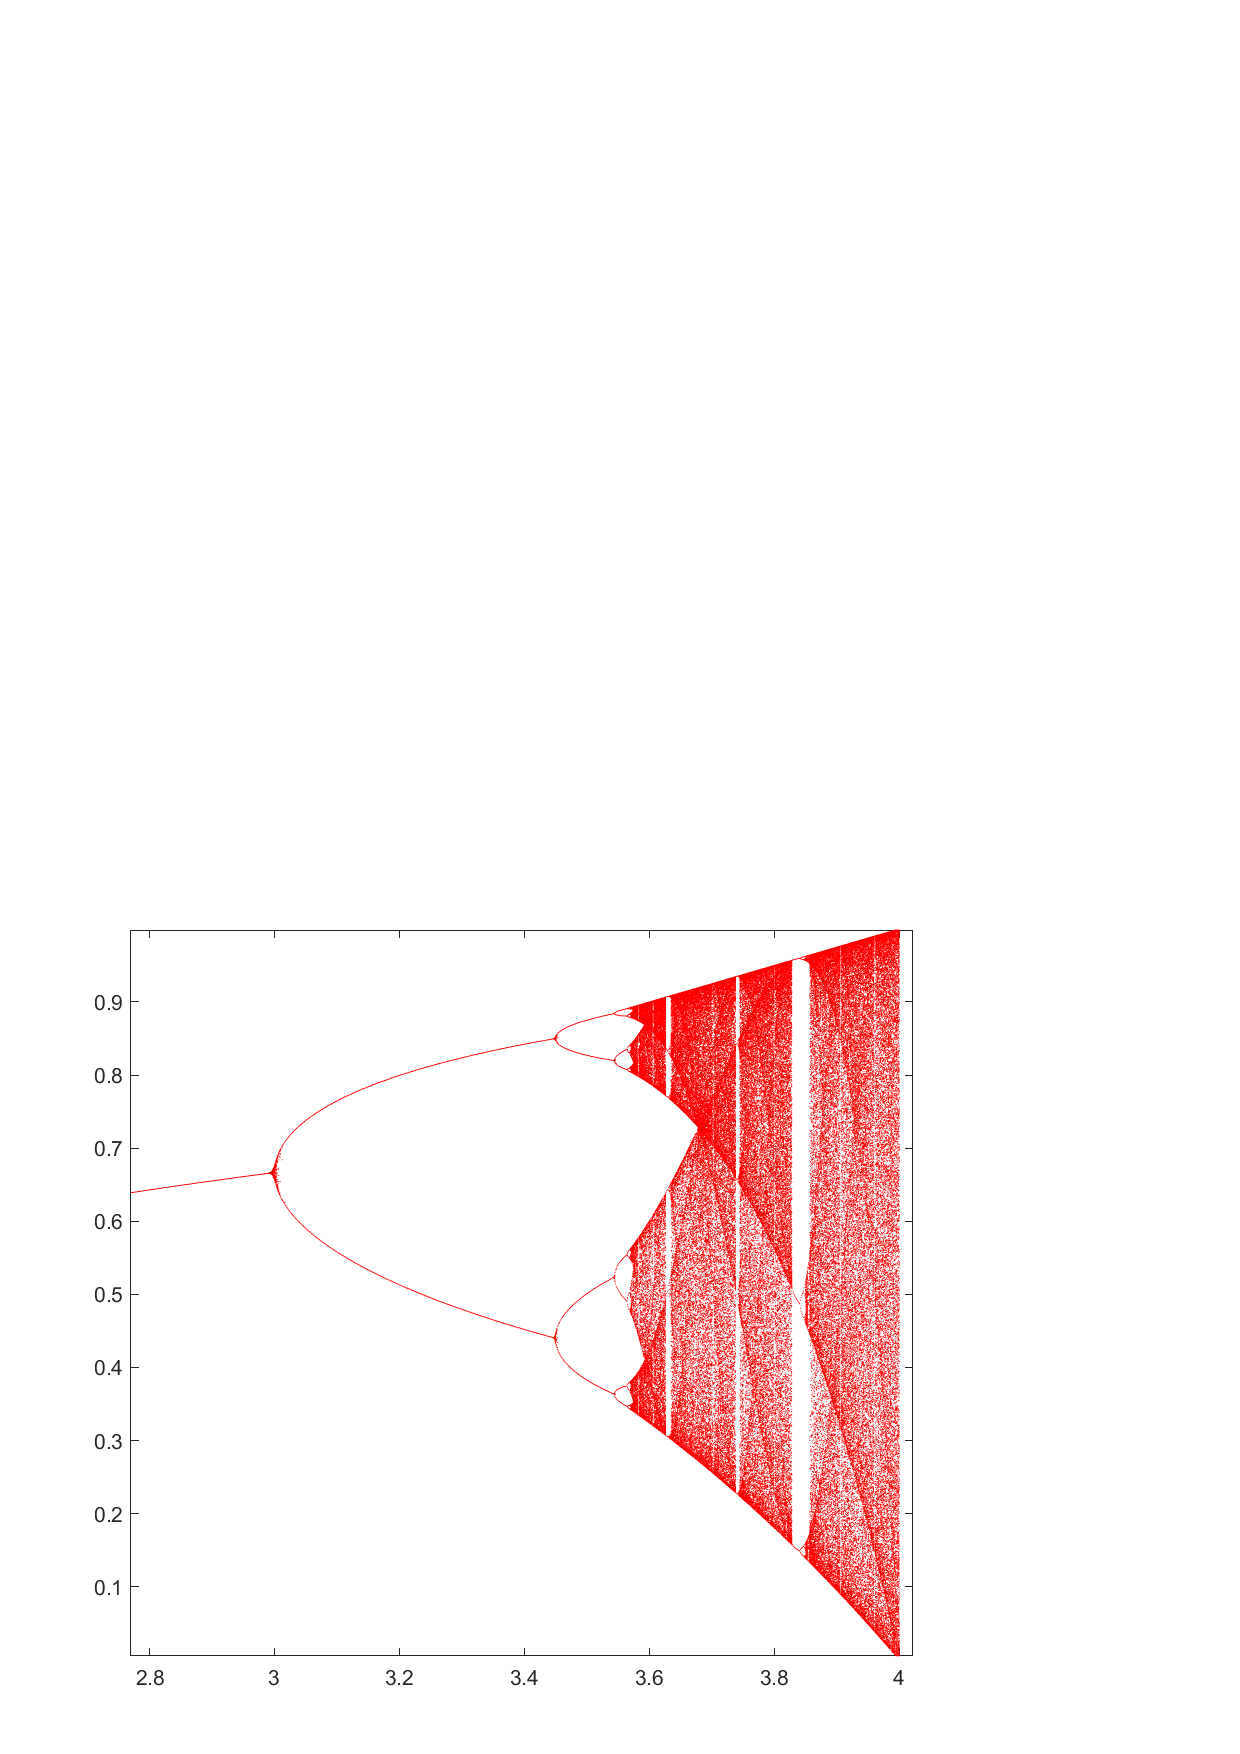
\includegraphics[scale=0.4]{logistic_1}
	\caption{Bifurcation diagram, for $2.8 \leq a \leq 4$.}
	\label{fig:logistic_1}
\end{figure}
\begin{figure}[!htb]
	\centering
	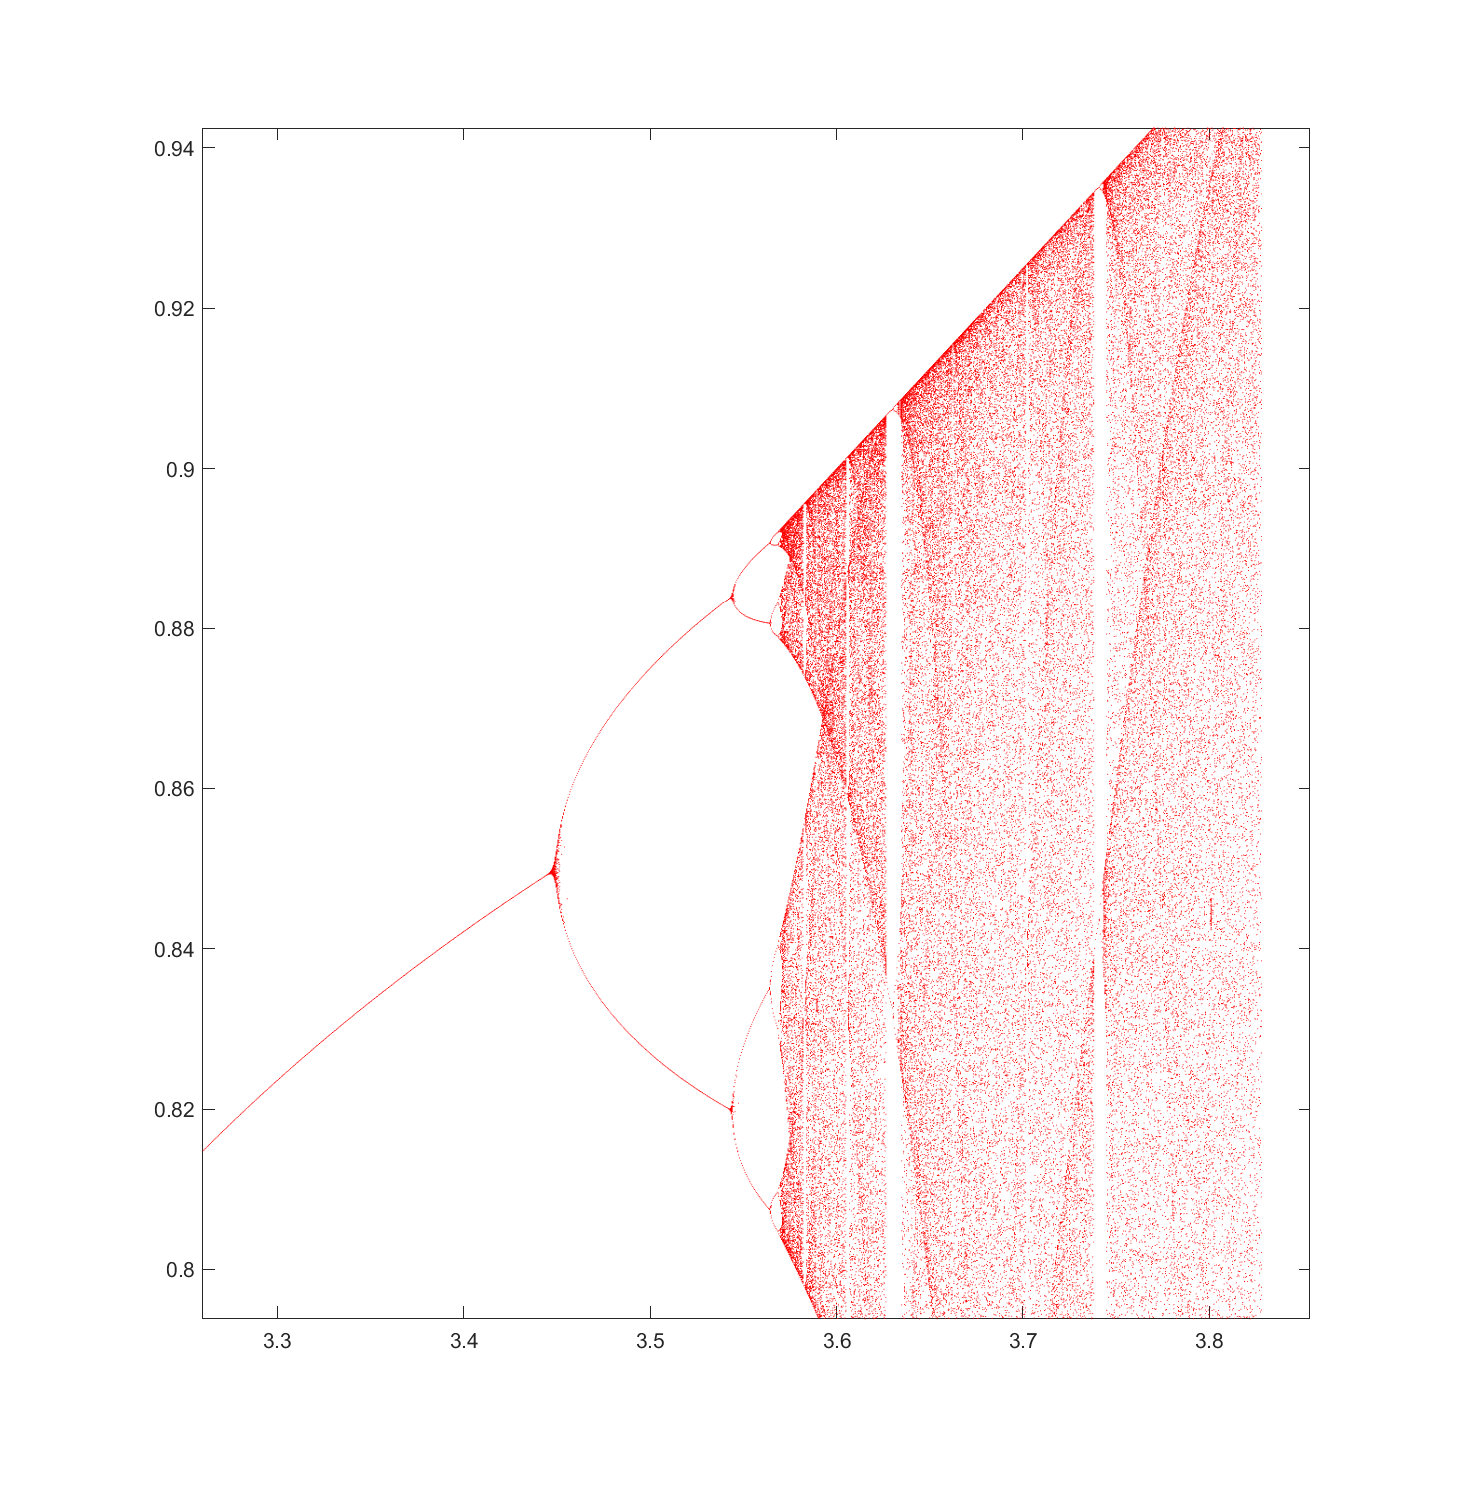
\includegraphics[scale=0.3]{logistic_3}
	\caption{Bifurcation diagram, for $3.3 \leq a \leq 3.8$}
	\label{fig:logistic_3}
\end{figure}
\begin{figure}[!htb]
	\centering
	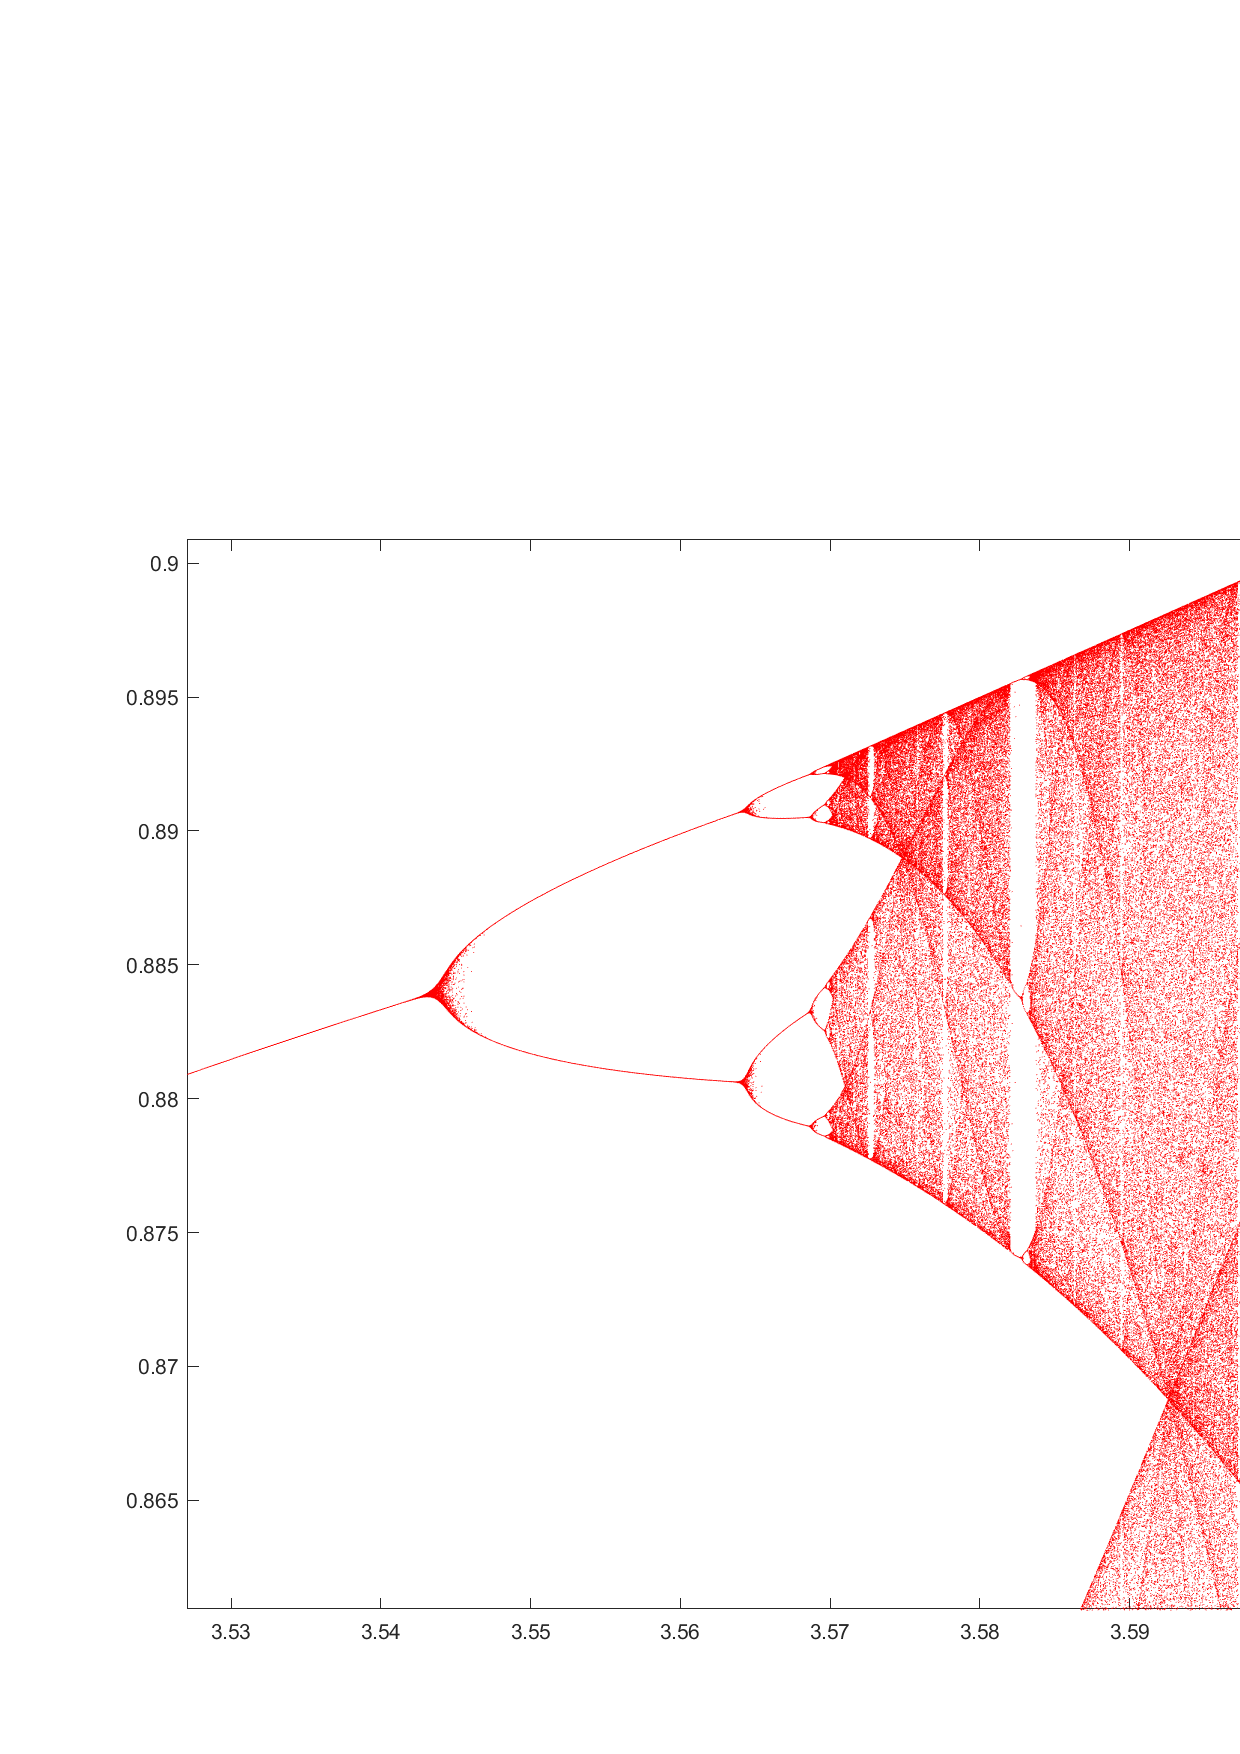
\includegraphics[scale=0.3]{logistic_4_top_branch_1}
	\caption{Bifurcation diagram, for $3.53 \leq a \leq 3.6$.}
	\label{fig:logistic_4}
\end{figure}
\begin{figure}[!htb]
	\centering
	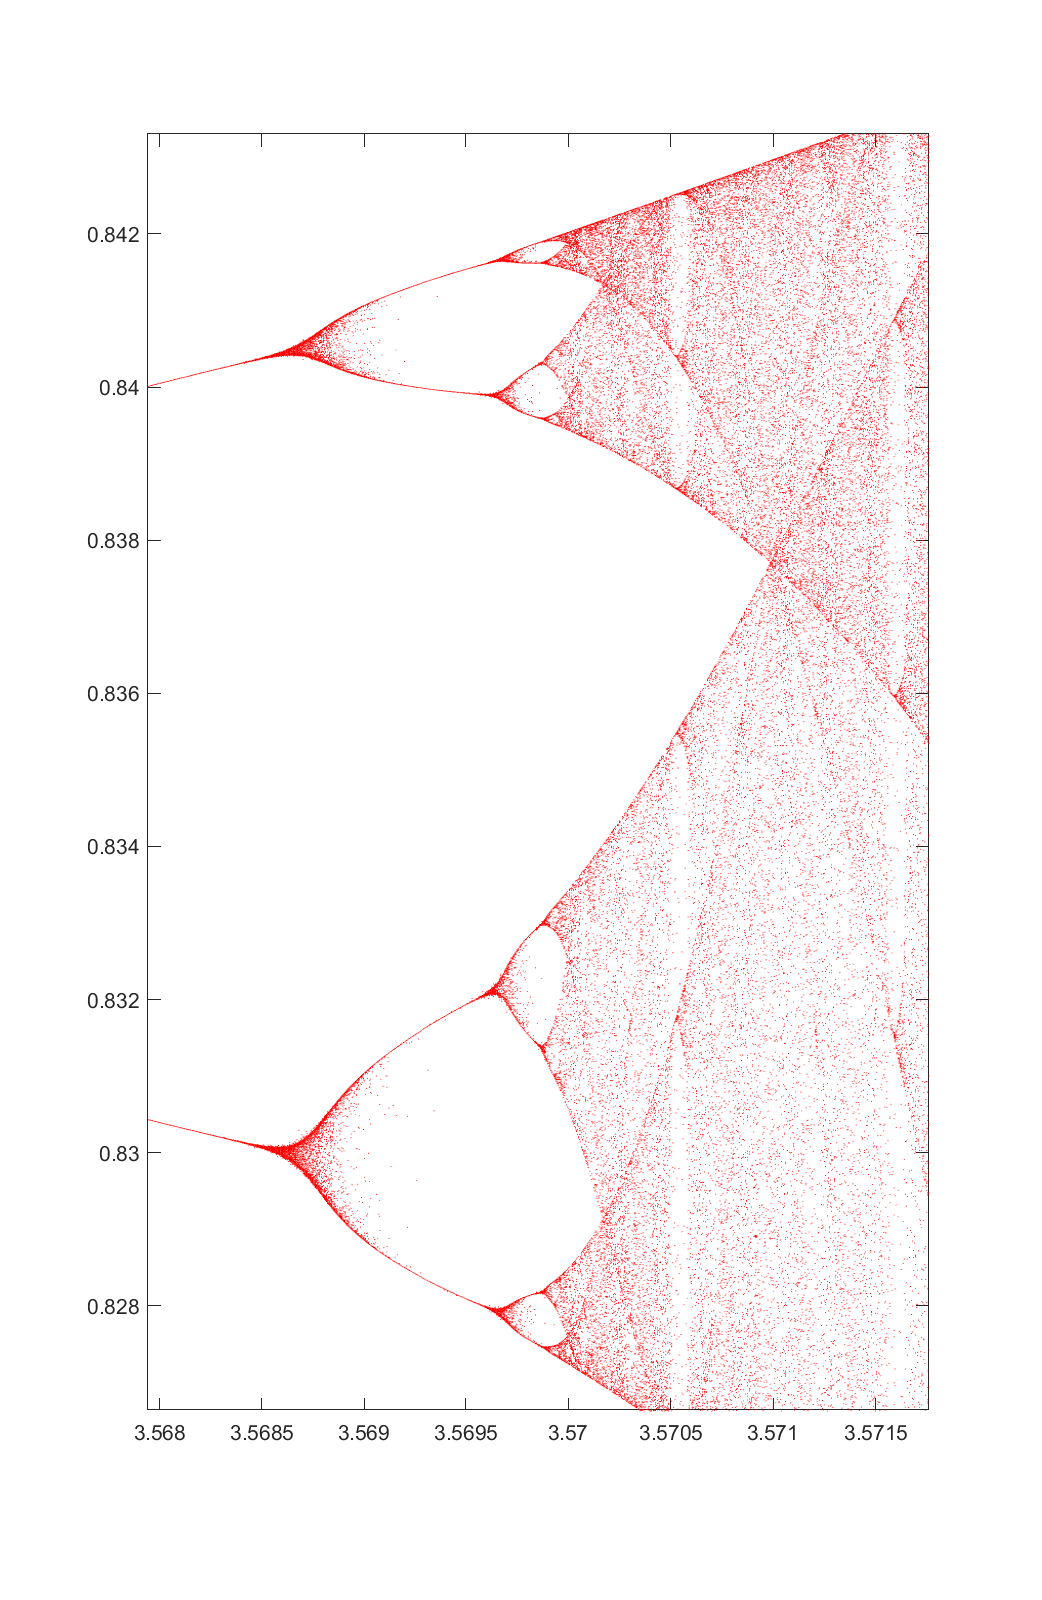
\includegraphics[scale=0.35]{logistic_5_more_branches}
	\caption{Bifurcation diagram, for $3.568 \leq a \leq 3.5715$.}
	\label{fig:logistic_5}
\end{figure}


%\begin{figure}[!htb]
%	\centering
%	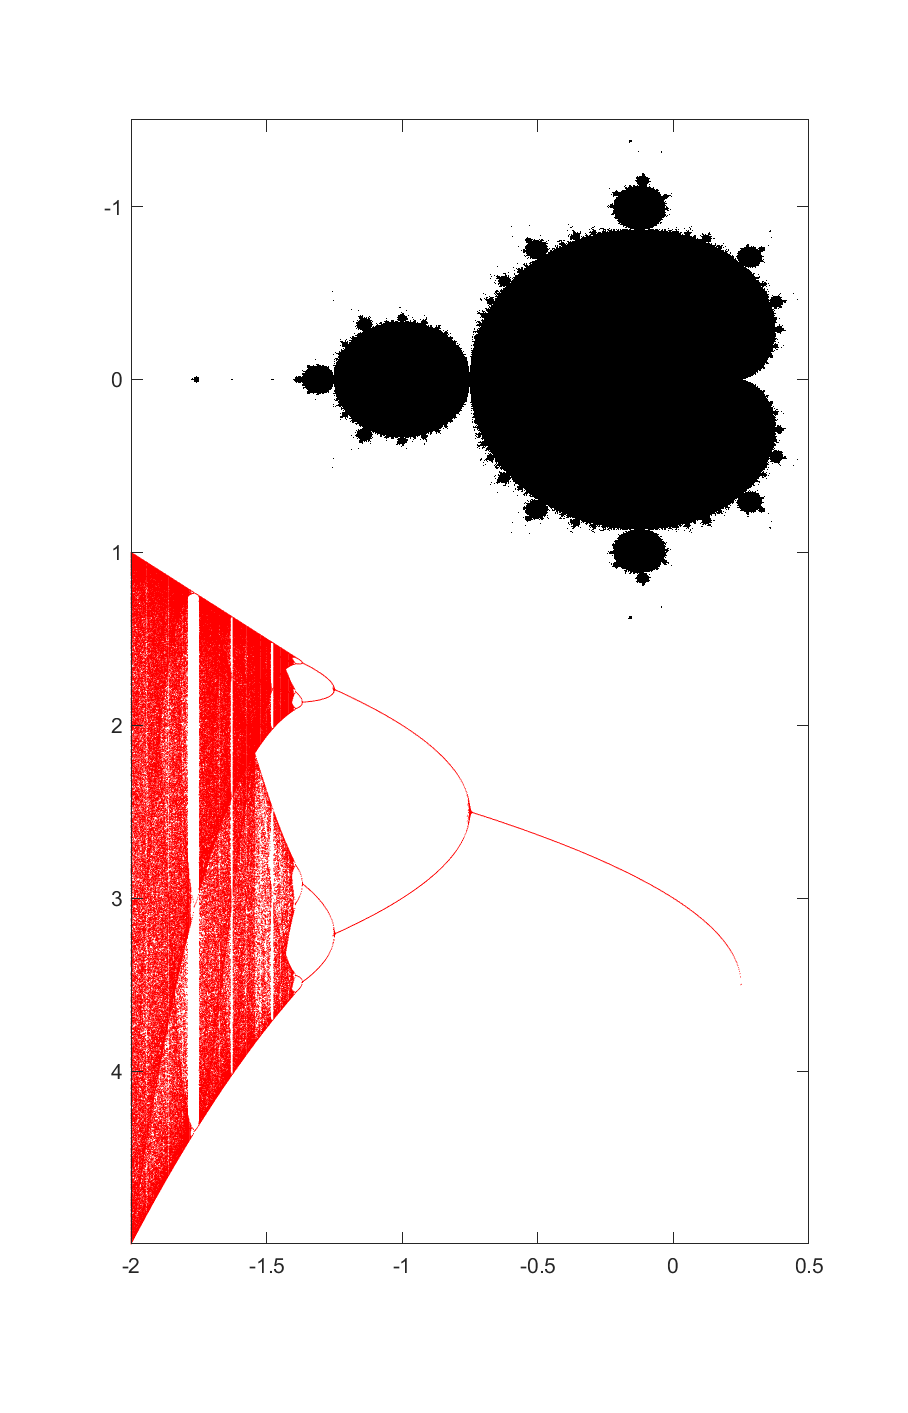
\includegraphics[scale=0.5]{mandelbrot_1}
%	\caption{Bifurcation diagram and the Mandelbrot set}
%	\label{fig:mandelbrot}
%\end{figure}





\section{Summary}

\textcolor{red}{I don't know why the formatting is doing all this line-skipping weirdness... This is really bothering me, but I'm too tired and can't be bothered to fix it now.}


Through the Lorenz system and the Robert May's work on a simple example of the logistic map, we saw a fascinating connection between \textit{order} and \textit{chaos} in nonlinear science. We learned that chaos is not strictly random and unpredictable. We developed a more nuanced way to characterize chaos as deterministic, but extremely sensitive to changes in initial condition. The strange attractor captures these two notions. We also found that chaotic systems do not necessarily behave in a truly random fashion. Rather, it is possible to have an underlying regularity in the seemingly chaotic behaviors. This is evident through the analysis of the Poincar\'{e} section of the Lorenz system. Finally, we saw that it is also possible to generate chaotic behavior by first setting a Poincar\'{e} section (which needs not be very complicated). This is the essence of Robert May's 1976 discovery.


\bibliography{paper2}


\end{document}